\documentclass[tikz,border=12pt]{standalone}
\usepackage{amsmath,amssymb}
\usetikzlibrary{calc,arrows.meta}

\begin{document}
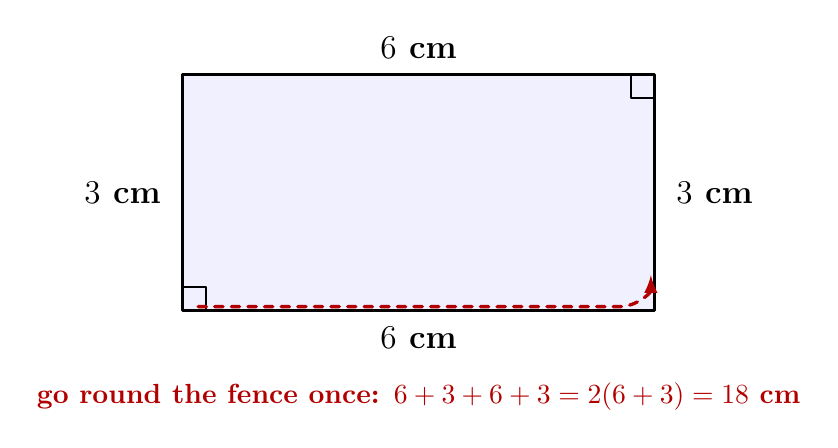
\begin{tikzpicture}[>=latex, line cap=round, line join=round]

  % Rectangle 6 by 3
  \draw[very thick, fill=blue!6] (0,0) rectangle (6,3);

  % Side length labels
  \node[above, font=\large\bfseries] at (3,3.08) {$6$ cm};
  \node[below, font=\large\bfseries] at (3,-0.08) {$6$ cm};
  \node[left, font=\large\bfseries, rotate=0] at (-0.15,1.5) {$3$ cm};
  \node[right, font=\large\bfseries] at (6.15,1.5) {$3$ cm};

  % Right angle indicators at two opposite corners
  \draw[thick] (0,0.3) -- (0.3,0.3) -- (0.3,0);
  \draw[thick] (6,2.7) -- (5.7,2.7) -- (5.7,3);

  % Perimeter sweep arrow along the boundary
  \draw[very thick, red!70!black, dashed, ->]
    (0.2,0.05) -- (5.55,0.05) to[out=0,in=270] (5.95,0.45);
  \node[red!70!black, font=\bfseries, below=2pt] at (3,-0.72)
    {go round the fence once: $6+3+6+3 = 2(6+3) = 18$ cm};

\end{tikzpicture}
\end{document}
